\documentclass[border=4pt,12pt]{standalone}
% House style for redrawn exam diagrams (diagram-v4: 0.4pt lines, filled -latex arrows, fine dashes; stipple and hatching drawn as real dots/lines (no PDF/SVG patterns, so they render in every browser and at any scale); transparent background). Every figure \input's this.
\usepackage{amsmath,amssymb}
\usepackage{txfonts}
\usepackage{pdfrender,xcolor}
% \halo{text}: label on shading. The shading stops just around each letter's outline (a thin knock-out that follows the
% glyphs, like the papers' typesetting), never a box. Owner: "I don't want a box around the text".
\newcommand{\halo}[1]{\leavevmode\rlap{\pdfrender{TextRenderingMode=2,LineWidth=2.2pt,LineJoinStyle=1,StrokeColor=white,FillColor=white}#1}#1}
\usepackage{tikz,pgfplots}
\pgfplotsset{compat=1.18}
\usetikzlibrary{arrows.meta,calc,angles,quotes,patterns,patterns.meta,intersections,positioning,decorations.markings,shapes.geometric}
% Stipple and hatching are drawn as actual dots / lines clipped to the region (path picture), NOT as pattern fills:
% SVG <pattern> fills vanish or blur when browsers scale the image, so the owner could not see the shading.
% Each dot is a 0.72pt square (keeps SVGs small; reads as a dot at print size). Dots sit on one global staggered grid, so neighbouring regions line up.
\makeatletter
\newdimen\ex@x \newdimen\ex@y \newdimen\ex@xa \newdimen\ex@ya \newdimen\ex@xb \newdimen\ex@yb \newcount\ex@row
\def\exam@stipplecolor{black!75}\def\exam@dotr{0.42pt}\def\exam@dotgap{2.5}
\def\ex@rowdots{\ifdim\ex@x<\ex@xb \pgfpathrectangle{\pgfqpoint{\dimexpr\ex@x-0.36pt\relax}{\dimexpr\ex@y-0.36pt\relax}}{\pgfqpoint{0.72pt}{0.72pt}}\advance\ex@x by \exam@dotgap pt\relax\expandafter\ex@rowdots\fi}
\def\exam@stipple{%
  \pgftransformreset% dots are sized in real points even inside scaled pictures
  \pgfpointanchor{path picture bounding box}{south west}\ex@xa=\pgf@x \ex@ya=\pgf@y
  \pgfpointanchor{path picture bounding box}{north east}\ex@xb=\pgf@x \ex@yb=\pgf@y
  \pgfsetfillcolor{\exam@stipplecolor}\pgfmathsetmacro\ex@h{\exam@dotgap/2}%
  \pgfmathtruncatemacro\ex@r{floor(\ex@ya/\ex@h)-1}\ex@row=\ex@r\relax
  \ex@y=\ex@r\dimexpr\ex@h pt\relax
  \loop\ifdim\ex@y<\ex@yb
    \pgfmathtruncatemacro\ex@c{floor(\ex@xa/\exam@dotgap)-1}\ex@x=\ex@c\dimexpr\exam@dotgap pt\relax
    \ifodd\ex@row \advance\ex@x by \ex@h pt\fi
    \ex@rowdots
    \advance\ex@y by \ex@h pt \advance\ex@row by 1
    \ifnum\numexpr\ex@row-(\ex@row/4)*4\relax=0 \pgfusepath{fill}\fi% flush every 4 rows: bounded TeX memory, few clip copies in the SVG
  \repeat\pgfusepath{fill}}
\newdimen\ex@d
\def\exam@hatch#1{% #1 = 1 for /, -1 for \ ; lines 45 degrees, 3pt apart
  \pgftransformreset
  \pgfpointanchor{path picture bounding box}{south west}\ex@xa=\pgf@x \ex@ya=\pgf@y
  \pgfpointanchor{path picture bounding box}{north east}\ex@xb=\pgf@x \ex@yb=\pgf@y
  \ex@d=\dimexpr\ex@yb-\ex@ya\relax \ex@x=\dimexpr\ex@xa-\ex@d\relax
  \loop\ifdim\ex@x<\ex@xb
    \ifnum#1>0 \pgfpathmoveto{\pgfqpoint{\ex@x}{\ex@ya}}\pgfpathlineto{\pgfqpoint{\dimexpr\ex@x+\ex@d\relax}{\ex@yb}}%
    \else \pgfpathmoveto{\pgfqpoint{\ex@x}{\ex@yb}}\pgfpathlineto{\pgfqpoint{\dimexpr\ex@x+\ex@d\relax}{\ex@ya}}\fi
    \advance\ex@x by 4.24pt
  \repeat
  \pgfsetlinewidth{0.4pt}\pgfsetstrokecolor{black}\pgfusepath{stroke}}
\def\examstipple{\exam@stipple}\def\examhatch{\exam@hatch}\def\examsetstipplecolor#1{\def\exam@stipplecolor{#1}}\def\examsetdotgap#1{\def\exam@dotgap{#1}}
\makeatother
% (legacy pattern kept for old files)
% staggered stipple like the NESA papers' dotted shading
\pgfdeclarepatternformonly{exam stipple}{\pgfpointorigin}{\pgfqpoint{2.2pt}{2.2pt}}{\pgfqpoint{2.2pt}{2.2pt}}{%
  \pgfpathcircle{\pgfqpoint{0.55pt}{0.55pt}}{0.42pt}\pgfpathcircle{\pgfqpoint{1.65pt}{1.65pt}}{0.42pt}\pgfusepath{fill}}
\tikzset{
  every picture/.style={line width=0.6pt, >={Latex[length=2mm,width=1.3mm]}},
  curve/.style={line width=0.6pt},
  open arrow/.style={-{Latex[length=2mm,width=1.3mm]}},  % owner: filled -latex heads everywhere, no open chevrons
  aux/.style={dash pattern=on 2pt off 1.5pt, line width=0.6pt},
  shade/.code={\def\exA{#1}\def\exB{none}\ifx\exA\exB\else\pgfkeysalso{fill=black!18}\fi},
  shade/.default=on,
  shade dots/.style={fill=none, path picture={\examstipple}},
  stipple color/.code={\examsetstipplecolor{#1}},
  stipple gap/.code={\examsetdotgap{#1}},
  shade dense dots/.style={fill=none, stipple gap=1.6, path picture={\examstipple}},
  shade hatch/.style={fill=none, path picture={\examhatch{1}}},
  shade hatch reverse/.style={fill=none, path picture={\examhatch{-1}}},
  shade solid/.style={fill=black},
  pt/.style={circle, fill, inner sep=1.1pt},
  open pt/.style={circle, draw, fill=white, inner sep=1.1pt},
}
\pgfplotsset{
  exam axes/.style={axis lines=middle, axis line style={->}, xlabel={$x$}, ylabel={$y$},
    xlabel style={anchor=west}, ylabel style={anchor=south}, tick label style={font=\small},
    every axis plot/.append style={line width=0.6pt, black}, samples=200, clip=false,
    enlargelimits=false, axis on top},
}

\begin{document}
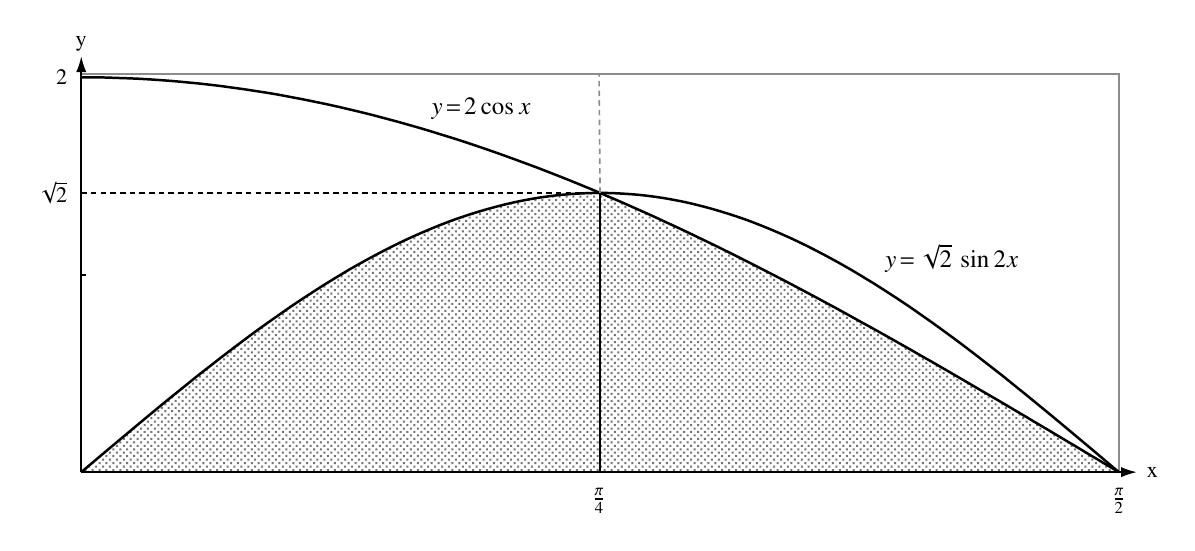
\begin{tikzpicture}[x=0.0127cm,y=-0.0127cm]
\fill[shade dots,stipple color=black!55] plot[smooth] coordinates {(44.0,452.0) (55.8,442.0) (67.6,432.1) (79.4,422.1) (91.2,412.3) (103.0,402.4) (114.8,392.6) (126.6,382.9) (138.4,373.3) (150.2,363.8) (162.0,354.4) (173.7,345.1) (185.5,336.0) (197.3,327.0) (209.1,318.1) (220.9,309.5) (232.7,301.0) (244.5,292.7) (256.3,284.6) (268.1,276.7) (279.9,269.1) (291.7,261.7) (303.5,254.5) (315.3,247.6) (327.1,240.9) (338.9,234.5) (350.7,228.4) (362.5,222.6) (374.3,217.0) (386.1,211.8) (397.9,206.9) (409.7,202.2) (421.4,197.9) (433.2,194.0) (445.0,190.3) (456.8,187.0) (468.6,184.0) (480.4,181.4) (492.2,179.1) (504.0,177.1) (515.8,175.5) (527.6,174.3) (539.4,173.4) (551.2,172.9) (563.0,172.7) (574.8,177.7) (586.6,182.8) (598.4,188.0) (610.2,193.3) (622.0,198.7) (633.8,204.1) (645.6,209.7) (657.4,215.3) (669.1,221.0) (680.9,226.7) (692.7,232.5) (704.5,238.4) (716.3,244.4) (728.1,250.4) (739.9,256.5) (751.7,262.7) (763.5,268.9) (775.3,275.2) (787.1,281.5) (798.9,287.9) (810.7,294.4) (822.5,300.8) (834.3,307.4) (846.1,314.0) (857.9,320.6) (869.7,327.3) (881.5,334.0) (893.3,340.7) (905.1,347.5) (916.8,354.3) (928.6,361.2) (940.4,368.0) (952.2,374.9) (964.0,381.9) (975.8,388.8) (987.6,395.8) (999.4,402.8) (1011.2,409.8) (1023.0,416.8) (1034.8,423.8) (1046.6,430.9) (1058.4,437.9) (1070.2,444.9) (1082.0,452.0)} -- cycle;
\draw[black!45] (44,54) -- (1082,54) -- (1082,452);
\draw[->] (44,452) -- (1100,452) node[right=0pt,font=\footnotesize] {x};
\draw[->] (44,452) -- (44,36) node[above=-2pt,font=\footnotesize] {y};
\draw (44,254.5) -- ++(5,0);
\draw[line width=0.9pt] plot[smooth] coordinates {(44.0,452.0) (55.7,442.1) (67.3,432.3) (79.0,422.5) (90.7,412.7) (102.3,403.0) (114.0,393.3) (125.6,383.7) (137.3,374.2) (149.0,364.8) (160.6,355.4) (172.3,346.3) (184.0,337.2) (195.6,328.3) (207.3,319.5) (218.9,310.9) (230.6,302.5) (242.3,294.3) (253.9,286.2) (265.6,278.4) (277.3,270.8) (288.9,263.4) (300.6,256.3) (312.2,249.3) (323.9,242.7) (335.6,236.3) (347.2,230.2) (358.9,224.3) (370.6,218.7) (382.2,213.5) (393.9,208.5) (405.5,203.8) (417.2,199.4) (428.9,195.4) (440.5,191.7) (452.2,188.3) (463.9,185.2) (475.5,182.4) (487.2,180.0) (498.8,177.9) (510.5,176.2) (522.2,174.8) (533.8,173.8) (545.5,173.1) (557.2,172.7) (568.8,172.7) (580.5,173.1) (592.1,173.8) (603.8,174.8) (615.5,176.2) (627.1,177.9) (638.8,180.0) (650.5,182.4) (662.1,185.2) (673.8,188.3) (685.4,191.7) (697.1,195.4) (708.8,199.4) (720.4,203.8) (732.1,208.5) (743.8,213.5) (755.4,218.7) (767.1,224.3) (778.8,230.2) (790.4,236.3) (802.1,242.7) (813.7,249.3) (825.4,256.3) (837.1,263.4) (848.7,270.8) (860.4,278.4) (872.1,286.2) (883.7,294.3) (895.4,302.5) (907.0,310.9) (918.7,319.5) (930.4,328.3) (942.0,337.2) (953.7,346.3) (965.4,355.4) (977.0,364.8) (988.7,374.2) (1000.3,383.7) (1012.0,393.3) (1023.7,403.0) (1035.3,412.7) (1047.0,422.5) (1058.7,432.3) (1070.3,442.1) (1082.0,452.0)};
\draw[line width=0.9pt] plot[smooth] coordinates {(44.0,57.0) (55.7,57.1) (67.3,57.2) (79.0,57.6) (90.7,58.0) (102.3,58.5) (114.0,59.2) (125.6,60.0) (137.3,60.9) (149.0,62.0) (160.6,63.1) (172.3,64.4) (184.0,65.8) (195.6,67.4) (207.3,69.0) (218.9,70.8) (230.6,72.6) (242.3,74.6) (253.9,76.8) (265.6,79.0) (277.3,81.4) (288.9,83.8) (300.6,86.4) (312.2,89.1) (323.9,91.9) (335.6,94.8) (347.2,97.9) (358.9,101.0) (370.6,104.3) (382.2,107.6) (393.9,111.1) (405.5,114.7) (417.2,118.3) (428.9,122.1) (440.5,126.0) (452.2,130.0) (463.9,134.1) (475.5,138.3) (487.2,142.6) (498.8,146.9) (510.5,151.4) (522.2,156.0) (533.8,160.6) (545.5,165.4) (557.2,170.2) (568.8,175.2) (580.5,180.2) (592.1,185.3) (603.8,190.5) (615.5,195.7) (627.1,201.1) (638.8,206.5) (650.5,212.0) (662.1,217.6) (673.8,223.2) (685.4,228.9) (697.1,234.7) (708.8,240.6) (720.4,246.5) (732.1,252.5) (743.8,258.5) (755.4,264.6) (767.1,270.8) (778.8,277.0) (790.4,283.3) (802.1,289.6) (813.7,296.0) (825.4,302.5) (837.1,308.9) (848.7,315.4) (860.4,322.0) (872.1,328.6) (883.7,335.3) (895.4,341.9) (907.0,348.6) (918.7,355.4) (930.4,362.2) (942.0,369.0) (953.7,375.8) (965.4,382.6) (977.0,389.5) (988.7,396.4) (1000.3,403.3) (1012.0,410.2) (1023.7,417.2) (1035.3,424.1) (1047.0,431.1) (1058.7,438.1) (1070.3,445.0) (1082.0,452.0)};
\draw (563.0,452.0) -- (563.0,172.7);
\draw[aux] (44.0,172.7) -- (563.0,172.7);
\draw[aux,black!45] (563.0,172.7) -- (562,54);
\node[font=\footnotesize,anchor=east] at (40,57) {2};
\node[font=\footnotesize,anchor=east] at (40,172.7) {$\sqrt{2}$};
\node[font=\small,anchor=north] at (562,458) {$\frac{\pi}{4}$};
\node[font=\small,anchor=north] at (1082,458) {$\frac{\pi}{2}$};
\node[font=\small] at (444,88) {$y\!=\!2\cos x$};
\node[font=\small] at (915,238) {$y\!=\!\sqrt{2}\,\sin 2x$};
\end{tikzpicture}
\end{document}
